\tikzstyle{knight}=[draw, shape=circle, fill=white]
\tikzstyle{jump}=[->, thick]
\tikzstyle{odd}=[black!40!red]
\tikzstyle{even}=[black!60]
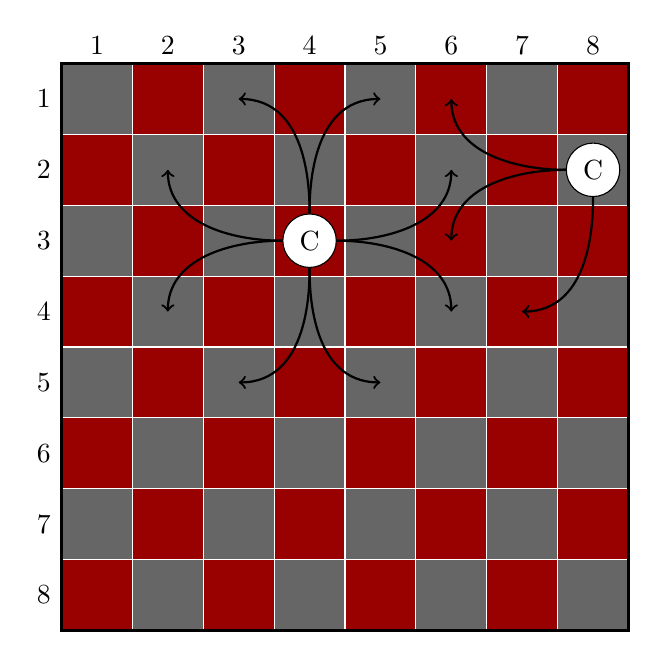
\begin{tikzpicture}[yscale=-1, scale=.9]
  \foreach\n in {1,...,8} {
    \node at (-.25, \n - .5) {\n};
    \node at (\n - .5, -.25) {\n};
  }
  \foreach\row in {0,2,4,6} {
    \foreach\col in {1,3,5,7} {
      \fill[odd]  (\row, \col)     rectangle ++(1, 1);
      \fill[even] (\row, \col - 1) rectangle ++(1, 1);
    }
  }
  \foreach\row in {1,3,5,7} {
    \foreach\col in {0,2,4,6} {
      \fill[odd]  (\row, \col) rectangle ++(1, 1);
      \fill[even] (\row, \col + 1) rectangle ++(1, 1);
    }
  }
  \draw[white] (0, 0) grid      ++(8, 8);
  \draw[thick] (0, 0) rectangle ++(8, 8);

  \def\row{2}
  \def\col{8}
  \node[knight] (c1) at (\col - .5, \row - .5) {C};
  \draw [jump, out=180, in= 90] (c1) to (\col - 2 - .5, \row - 1 - .5);
  \draw [jump, out=180, in=-90] (c1) to (\col - 2 - .5, \row + 1 - .5);
  \draw [jump, out= 90, in=  0] (c1) to (\col - 1 - .5, \row + 2 - .5);

  \def\row{3}
  \def\col{4}
  \node[knight] (c1) at (\col - .5, \row - .5) {C};
  \draw [jump, out=180, in= 90] (c1) to (\col - 2 - .5, \row - 1 - .5);
  \draw [jump, out=180, in=-90] (c1) to (\col - 2 - .5, \row + 1 - .5);
  \draw [jump, out=-90, in=  0] (c1) to (\col - 1 - .5, \row - 2 - .5);
  \draw [jump, out= 90, in=  0] (c1) to (\col - 1 - .5, \row + 2 - .5);
  \draw [jump, out=  0, in= 90] (c1) to (\col + 2 - .5, \row - 1 - .5);
  \draw [jump, out=  0, in=-90] (c1) to (\col + 2 - .5, \row + 1 - .5);
  \draw [jump, out=-90, in=180] (c1) to (\col + 1 - .5, \row - 2 - .5);
  \draw [jump, out= 90, in=180] (c1) to (\col + 1 - .5, \row + 2 - .5);

\end{tikzpicture}

